\documentclass[compress,9pt]{beamer} % TALK

\usepackage{pgfpages}

%\setbeameroption{hide notes} % solo muestra la presentación.
%\setbeameroption{show only notes} % solo muestras las notas.
%\setbeameroption{show notes on second screen=right} % presentación el doble de ancha que contiene las diapositivas y las notas. 


\usepackage{tikz}   %TikZ is required for this to work.  Make sure this exists before the next line

\usepackage{tikz-3dplot} %requires 3dplot.sty to be in same directory, or in your LaTeX installation

\usetikzlibrary{babel}

% tikz-3dplot-circleofsphere: To draw 3D spheres ----------
\usepackage{tikz-3dplot-circleofsphere} %requires tikz-3dplot-circleofsphere to be in same directory, or in your LaTeX installation



\begin{document}
	
	\section{Physics: Newton's and Kepler's dynamics.}
	\begin{frame}[fragile,label={frm:newtonGravit}]{Newton's law of universal gravitation}
		%requires tikz-3dplot-circleofsphere to be in same directory, or in your LaTeX installation
		% Figure: Universal gravity law
		\begin{figure}[H]
			\centering
			% Select a perspective
			\tdplotsetmaincoords{75}{115}
			\begin{tikzpicture}[scale=1,tdplot_main_coords,>=latex,line join=bevel]
			% Parameters ---------------------
			% Coordinates parameters
			\pgfmathsetmacro{\sizeCoordX}{5.2*.6}
			\pgfmathsetmacro{\sizeCoordY}{5.2*.6}
			\pgfmathsetmacro{\sizeCoordZ}{4.2*.6}
			\coordinate (O) at (0,0,0);
			
			% m satellite position parameters
			\pgfmathsetmacro{\mx}{.7 * \sizeCoordX}
			\pgfmathsetmacro{\my}{0.9 * \sizeCoordY}
			\pgfmathsetmacro{\mz}{0.7 * \sizeCoordZ}
			
			% It is very important to get redundant parenthesis
			% Radius = rho
			\pgfmathsetmacro{\mr}{sqrt{((\mx)^2 + (\my)^2 + (\mz)^2)}}
			% theta = epsilon
			% \pgfmathsetmacro{\mEpsilon}{acos{ ( (\mz)/(\mr) ) }}
			\pgfmathsetmacro{\mEpsilon}{atan{(sqrt{((\mx)^2 + (\my)^2)}/(\mz))}}
			% phi = alpha
			\pgfmathsetmacro{\mAlpha}{atan{((\my) / (\mx))}}
			% polar angle = beta
			\pgfmathsetmacro{\mBeta}{atan{((\mz) / (sqrt{((\mx)^2 + (\my)^2)}))}}
			
			% Debug info
			% \node [label={right:\mr}] at (0, 0, -3) {mr};
			% \node [label={right:\mEpsilon}] at (0, 0, -4) {mEpsilon};
			% \node [label={right:\mAlpha}] at (0, 0, -5) {mAlpha};
			% \node [label={right:\mBeta}] at (0, 0, -6) {mBeta};
			
			% Little mass size
			\pgfmathsetmacro{\mSize}{15}
			
			% M Earth parameters
			\pgfmathsetmacro{\radiusXY}{.22 * \sizeCoordX}
			\pgfmathsetmacro{\radiusZ}{.19 * \sizeCoordX}
			
			% Fg parameters
			\pgfmathsetmacro{\FgX}{.3 * \mx}
			\pgfmathsetmacro{\FgY}{.3 * \my}
			\pgfmathsetmacro{\FgZ}{.3 * \mz}
			
			% Figures ---------------------
			% Circle M Earth.
			\begin{scope}
			\filldraw[tdplot_screen_coords, gray!30] (0,0,0) circle (\radiusXY);
			\tdplotCsDrawLatCircle[gray]{\radiusXY}{0}
			\end{scope}
			%\node [label={left:$M_\oplus$}] at (0,-\radiusXY,\radiusZ) {};
			\node [anchor=south east] {$M_\oplus$};
			
			% Circle m satellite.
			\node [draw, circle, fill=gray!30, minimum size = \mSize, label=above:$m$] at (\mx, \my, \mz) {};
			
			% Satellite trajectory
			\tdplotCsDrawCircle[blue]{\mr}{\mAlpha}{-\mBeta}{0}
			\node [label={[blue]south east:Orbital plane}] at (0,\my,\mz) {};
			% Coordinates
			\draw[thick,->] (O) -- (\sizeCoordX,0,0) node[anchor=north east]{$x$};
			\draw[thick,->] (O) -- (0,\sizeCoordY,0) node[anchor=north west]{$y$};
			\draw[thick,->] (O) -- (0,0,0.8
			7*\sizeCoordZ) node[anchor=south]{$z$};
			\draw[dashed] (O) -- (-0.7*\sizeCoordX,0,0);
			\draw[dashed] (O) -- (0,-0.7*\sizeCoordY,0);
			% \draw[dashed] (O) -- (0,0,-\sizeCoordZ);
			
			% Satellite
			% r vector
			\draw[-stealth,color=blue,very thick] (0,0,0) -- (\mx,\my,\mz);
			\node [label={[blue]left:$\mathbf{r}$}] at (\mx/2, \my/2, \mz/2) {};
			% r Projection
			\draw[dotted] (0,0,0) -- (\mx,\my,0) --  (\mx,\my,\mz);
			\draw[dotted] (\mx,0,0) -- (\mx,\my,0) node[anchor=north east]{Equatorial plane};
			\draw[dotted] (\mx,\my,0) -- (0,\my,0);
			
			% F_g vector
			\draw[-stealth,color=blue,very thick] 
			(\FgX+\mx, \FgY+\my, \FgZ+\mz) -- (\mx, \my, \mz);
			% \node [label={[shift={(\mx+\Fg/2, \my+\Fg/2, \mz+\Fg/2)}]$\mathbf{F_g}$}] {};
			% \node [label={[blue]right:$\mathbf{F_g}$}] at (\mx+\FgX,\my+\FgY,\mz+\FgZ) {};
			\node [label={[blue]$\mathbf{F_g}$}] at (\mx+\FgX,\my+\FgY,\mz+\FgZ) {};
			\end{tikzpicture}
			%\caption{Newton's law of universal gravitation.} \label{fig:NewtonLaw}
		\end{figure}
		% Show equation
		\begin{equation}\label{eq:newton_gravity}
		\text{Newton's law of universal gravitation: } \mathbf{F_g} = -G\frac{{M_\oplus}{m}}{{r^2}}\left(\frac{\mathbf{r}}{r}\right)
		\end{equation}
	\end{frame}
	
	
	\begin{frame}[fragile]{Kepler's second law}
		\begin{figure}[H]
			\centering
			% Author: https://tex.stackexchange.com/questions/122122/best-way-to-illustrate-keplers-2nd-law-with-tikz
			% We define the orbit as a macro because we will use it twice, first for clipping and then
			% to actually draw the ellipse. This way we avoid inconsistencies.
			\def\orbit{(1.5,0) ellipse(2.5cm and 2cm)}
			
			\begin{tikzpicture}
			\fill (3,0) coordinate (O) circle (5pt) node[below left =7pt] {$M_\oplus$};%
			
			\coordinate (m1) at (0.90,2.30);
			\coordinate (m2) at (0.65,1.90);
			\coordinate (m3) at (3.5,-2.2);
			\coordinate (m4) at (4.0,-0.4);
			% Show m
			\fill (m2) circle (2pt) node[above left] {$m$};%
			
			% The gray shaded regions
			\begin{scope}
			\clip \orbit;
			\filldraw[fill=gray!40,opacity=0.5] (O) -- (m1) -- (m2) -- cycle;
			\filldraw[fill=gray!40,opacity=0.5] (O) -- (m3) -- (m4) -- cycle;
			\end{scope}
			
			% The ellipse
			\draw \orbit;
			% major and minor axis
			\draw[dashed] (1.5,0) coordinate (M) --node[above]{$a$}  (-1.0,0);
			\draw[dashed] (1.5,-2.0) -- (M) node[below left]{$b$};
			% true anomaly: nu
			\draw[-stealth,blue] (3.5,0) arc (0:140:0.5)node[above right]{$\nu$};
			\draw[dotted] (3,0) -- (4,0);
			\end{tikzpicture}
			\caption{Kepler's second law.}%\label{fig:Kepler2Law}
		\end{figure}
	\end{frame}
	
	% Orbital elements or Keplerian elements
	\begin{frame}[fragile,label={frm:elipse+}]
		% 
		\begin{figure}[H]
			\centering
			\def\r{3.5}
			\pgfmathsetmacro{\inclination}{35}
			\pgfmathsetmacro{\nuSatellite}{55}
			\pgfmathsetmacro{\gammaAngle}{290}
			
			\tdplotsetmaincoords{70}{165}
			\begin{tikzpicture}[tdplot_main_coords]
			\onslide<1->{
				\fill (0,0) coordinate (O) circle (5pt) node[left =7pt] {$M_\oplus$};
				
				% Draw equatorial ellipse
				%\tdplotdrawarc[thin]{(0,0,0)}{\r}{-90}{205}{label={[xshift=-3.7cm, yshift=0.9cm]Equatorial plane}}{}
				%\tdplotdrawarc[dotted]{(0,0,0)}{\r}{205}{270}{}{}
				% Draw equatorial plane
				\draw[] (0,-\r,0) -- (\r,-\r,0)  node[below]{Equatorial plane} -- (\r,\r,0) -- (-\r,\r,0) -- (-\r,-0.65*\r,0);
				\draw[dotted] (-\r,-0.65*\r,0) -- (-\r,-\r,0) -- (0,-\r,0);
				
				% Draw ellipses intersection. Line of nodes
				\draw[dashed] (0,-1.3*\r,0) -- (0,1.3*\r,0) node[right] {Line of nodes};
				% Draw gamma direction
			}
			
			\onslide<2->{
				% Set gamma direction
				\tdplotsetcoord{Pg}{1.3*\r}{90}{\gammaAngle}
				\draw[->] (0,0,0) -- (Pg) node[anchor=east] {Direcc. de referencia $\boldsymbol{\gamma}$};
			}
			\onslide<1->{
				% Create a new rotated system in the center
				\tdplotsetrotatedcoords{0}{\inclination}{90}
				
				% Draw orbital ellipse
				\tdplotdrawarc[tdplot_rotated_coords,thin,blue]{(0,0,0)}{\r}{-125}{180}{label={[xshift=-5.7cm, yshift=-2.2cm]Orbital plane}}{}
				\tdplotdrawarc[tdplot_rotated_coords,dotted,blue]{(0,0,0)}{\r}{180}{235}{}{}
				
				
				% Define m position
				\pgfmathsetmacro{\omegaSatellite}{90}
				\pgfmathsetmacro{\xmRot}{\r*cos(\omegaSatellite+\nuSatellite)}
				\pgfmathsetmacro{\ymRot}{\r*sin(\omegaSatellite+\nuSatellite)}
				\pgfmathsetmacro{\zmRot}{0}
				% Draw a vector to m
				\draw[tdplot_rotated_coords,thin,->,blue] (0,0,0) -- (\xmRot,\ymRot,\zmRot);
				% Draw a mass
				\filldraw[tdplot_rotated_coords, blue] (\xmRot,\ymRot,\zmRot) circle (2pt) node[above left] {$m$};
			}
			\onslide<5->{
				% Draw periapsis line
				\draw[dashed,tdplot_rotated_coords,blue] (0,0,0) -- (0,\r,0) node[anchor=south west] {Periapsis};
			}
			\onslide<5->{
				% Draw omega angle
				\tdplotdrawarc[tdplot_rotated_coords,thick,-stealth,blue]{(0,0,0)}{0.4*\r}{0}{\omegaSatellite}{anchor=south west}{$\omega$}
				% Draw nu angle
				\tdplotdrawarc[tdplot_rotated_coords,thick,-stealth,blue]{(0,0,0)}{0.4*\r}{\omegaSatellite}{\omegaSatellite+\nuSatellite}{anchor=south west}{$\nu$}
			}
			\onslide<3->{
				% Create rotated shifted system at (0,\r,0)
				\tdplotresetrotatedcoordsorigin
				\tdplotsetrotatedcoords{0}{0}{180}
				% Draw \Omega
				% Hidden part of the arc
				%% \tdplotdrawarc[tdplot_rotated_coords,dashed,thick,brown]{(0,0,0)}{0.4*\r}{0}{90}{anchor=south}{}%{$\Omega$}
				% Visible part of the arc
				\tdplotdrawarc[tdplot_rotated_coords,thick,-stealth,brown]{(0,0,0)}{0.4*\r}{\gammaAngle-180}{270}{anchor=north east}{$\Omega$}
				% Shift the rotated coordinates
				\coordinate (Shift) at (0,\r,0);
				\tdplotsetrotatedcoordsorigin{(Shift)}
				% \draw[thick,tdplot_rotated_coords,->,blue] (0,0,0) -- (.5,0,0) node[anchor=north west]{$x_2$};
				% \draw[thick,tdplot_rotated_coords,->,blue] (0,0,0) -- (0,.5,0) node[anchor=north]{$y_2$};
				% \draw[thick,tdplot_rotated_coords,->,blue] (0,0,0) -- (0,0,.5) node[anchor=south west]{$z_2$};
			}
			\onslide<4->{
				% Draw inclination angle
				\tdplotsetrotatedthetaplanecoords{0}
				\tdplotdrawarc[tdplot_rotated_coords,thick,-stealth,brown]{(Shift)}{0.3*\r}{90}{90-\inclination}{anchor=west}{$i$}
			}
			\end{tikzpicture}
			\caption{Orbital elements or Keplerian elements}\label{fig:elipseNodos2}
		\end{figure}	
	\end{frame}
	
	\section{Rotate a box around some axes.}
	\begin{frame}{Rotate box around $X$ axis.}
		\begin{figure}[h]
			\centering
			\def\r{3.5}
			\pgfmathsetmacro{\alphaNextBox}{90}
			\pgfmathsetmacro{\betaNextBox}{-55}
			\pgfmathsetmacro{\gammaNextBox}{-90}
			%%% \pgfmathsetmacro{\inclination}{70}
			\pgfmathsetmacro{\alphaEuler}{0}
			\pgfmathsetmacro{\betaEuler}{0}
			\pgfmathsetmacro{\gammaEuler}{47}
			
			\tdplotsetmaincoords{70}{120}
			\begin{tikzpicture}[tdplot_main_coords]
			% Drawing XYZ coordinates system
			\def \lenX {1.0*\r}
			\def \lenY {1.3*\r}
			\def \lenZ {1.0*\r}
			\def \boxX{.7*\r}
			\def \boxY{.9*\r}
			\def \boxZ{.2*\r}
			% Calculate box corner length
			\pgfmathsetmacro{\boxCornerLen}{sqrt{((\boxX)^2 + (\boxY)^2 + (\boxZ)^2)}}
			% Draw coordinate system
			\draw[dashed] (0,0,0) -- (\boxX,0,0);
			\draw[->,thick] (\boxX,0,0) -- (\lenX,0,0) node[left] {$X$};
			\draw[dashed] (0,0,0) -- (0,\boxY,0);
			\draw[->,thick] (0,\boxY,0) -- (0,\lenY,0) node[anchor=north west] {$Y$};
			\draw[dashed] (0,0,0) -- (0,0,0.6*\lenZ);
			\draw[->,thick] (0,0,0.6*\lenZ) -- (0,0,\lenZ) node[anchor=south] {$Z$};
			% Draw gravity vector
			\draw[-stealth,thin] (-0.8*\r,1.1*\r,0) -- (-0.8*\r,1.1*\r,-.3*\r) node[anchor=south west] {$\mathbf{g}$};
			
			% Drawing horizontal box:
			% Get corner polar coordinate
			\tdplotgetpolarcoords{\boxX}{\boxY}{\boxZ}
			\tdplotsetcoord{Box}{\boxCornerLen}{\tdplotrestheta}{\tdplotresphi}
			% Draw a box
			% \draw[] (O) -- (Boxx);
			% \draw[] (O) -- (Boxy);
			% \draw[] (O) -- (Boxz);
			\draw[] (Boxx) -- (Boxxy);
			\draw[] (Boxy) -- (Boxxy);
			\draw[] (Boxx) -- (Boxxz);
			\draw[] (Boxz) -- (Boxxz);
			\draw[] (Boxy) -- (Boxyz);
			\draw[] (Boxz) -- (Boxyz);
			\draw[] (Boxxy) -- (Box);
			\draw[] (Boxxz) -- (Box);
			\draw[] (Boxyz) -- (Box);
			\pause
			% Create a new rotated system in the center
			\tdplotsetrotatedcoords{\alphaEuler}{\betaEuler}{\gammaEuler}
			% Draw new coordinates system
			% Hidden line
			\draw[dashed,tdplot_rotated_coords,red] (0,0,0) -- (1.4*\boxX,0,0);
			% Visible line
			\draw[thick,tdplot_rotated_coords,->,red] (1.4*\boxX,0,0) -- (1.3*\lenX,0,0) node[anchor=north east]{$E$};
			% Hidden line
			\draw[dashed,tdplot_rotated_coords,red] (0,0,0) -- (0,0.7*\boxY,0);
			% Visible line
			\draw[thick,tdplot_rotated_coords,->,red] (0,0.7*\boxY,0) -- (0,0.8*\lenY,0) node[anchor=south west]{$\mathbf{N}$};
			% Hidden line
			\draw[dashed,tdplot_rotated_coords,red] (0,0,0) -- (0,0,0.6*\lenZ);
			% Visible line
			\draw[thick,tdplot_rotated_coords,->,red] (0,0,0.6*\lenZ) -- (0,0,0.8*\lenZ) node[anchor=north east]{$Z$};
			\pause
			% Rotating box around X axis:
			% Create a new rotated system in the center.
			\tdplotsetrotatedcoords{\alphaNextBox}{\betaNextBox}{\gammaNextBox}
			% Draw a box in the  new coordinates system
			\draw[tdplot_rotated_coords,gray] (\boxX,0,0) -- (\boxX,\boxY,0);
			\draw[tdplot_rotated_coords,gray] (\boxX,\boxY,0) -- (0,\boxY,0);
			\draw[tdplot_rotated_coords,gray] (0,\boxY,0) -- (0,\boxY,\boxZ);
			\draw[tdplot_rotated_coords,dashed,gray] (0,\boxY,\boxZ) -- (0,0,\boxZ);
			\draw[tdplot_rotated_coords,dashed,gray] (0,0,\boxZ) -- (\boxX,0,\boxZ);
			\draw[tdplot_rotated_coords,gray] (\boxX,0,\boxZ) -- (\boxX,0,0);
			\draw[tdplot_rotated_coords,gray] (\boxX,0,0) -- (\boxX,0,\boxZ);
			\draw[tdplot_rotated_coords,gray] (\boxX,0,\boxZ) -- (\boxX,\boxY,\boxZ);
			\draw[tdplot_rotated_coords,gray] (\boxX,\boxY,\boxZ) -- (0,\boxY,\boxZ);
			\draw[tdplot_rotated_coords,gray] (\boxX,\boxY,\boxZ) -- (\boxX,\boxY,0);
			\draw[tdplot_rotated_coords,dashed,gray] (0,0,\boxZ) -- (0,0,0);
			\draw[tdplot_rotated_coords,gray] (0,0,0) -- (0,\boxY,0);
			
			\tdplotsetrotatedcoordsorigin{(Shift)}
			% Shift the rotated coordinates
			\coordinate (Shift) at (\boxX,0,0);
			% Draw rotation
			\tdplotsetthetaplanecoords{90}
			% \tdplotdrawarc[coordinate system, draw styles]{center}{r}{angle start}{angle end}{label options}{label}
			\tdplotdrawarc[tdplot_rotated_coords,gray,thick,dotted,<->]{(Shift)}{\boxY}{90}{90+\betaNextBox}{anchor=west}{} 
			
			% Resets the origin of the rotated coordinate system back to the origin of the main coordinate system.
			%\tdplotresetrotatedcoordsorigin
			\coordinate (Shift) at (0,0,0);		
			\end{tikzpicture}
		\end{figure}
	\end{frame}
	
	
	\begin{frame}[fragile]{Rotate box around $Y$ axis.}
		\begin{figure}[h]
			\centering
			\def\r{3.5}
			\pgfmathsetmacro{\alphaNextBox}{0}%{90}
			\pgfmathsetmacro{\betaNextBox}{-50}%{-55}
			\pgfmathsetmacro{\gammaNextBox}{0}%{-90}
			%%% \pgfmathsetmacro{\inclination}{70}
			\pgfmathsetmacro{\alphaEuler}{0}
			\pgfmathsetmacro{\betaEuler}{0}
			\pgfmathsetmacro{\gammaEuler}{47}
			
			\tdplotsetmaincoords{70}{120}
			\begin{tikzpicture}[tdplot_main_coords]
			% Drawing XYZ coordinates system
			\def \lenX {1.0*\r}
			\def \lenY {1.3*\r}
			\def \lenZ {1.0*\r}
			\def \boxX{.7*\r}
			\def \boxY{.9*\r}
			\def \boxZ{.2*\r}
			% Calculate box corner length
			\pgfmathsetmacro{\boxCornerLen}{sqrt{((\boxX)^2 + (\boxY)^2 + (\boxZ)^2)}}
			% Draw coordinate system
			\draw[dashed] (0,0,0) -- (\boxX,0,0);
			\draw[->,thick] (\boxX,0,0) -- (\lenX,0,0) node[left] {$X$};
			\draw[dashed] (0,0,0) -- (0,\boxY,0);
			\draw[->,thick] (0,\boxY,0) -- (0,\lenY,0) node[anchor=north west] {$Y$};
			\draw[dashed] (0,0,0) -- (0,0,0.6*\lenZ);
			\draw[->,thick] (0,0,0.6*\lenZ) -- (0,0,\lenZ) node[anchor=south] {$Z$};
			% Draw gravity vector
			\draw[-stealth,thin] (-0.8*\r,1.1*\r,0) -- (-0.8*\r,1.1*\r,-.3*\r) node[anchor=south west] {$\mathbf{g}$};
			
			% Drawing horizontal box:
			% Get corner polar coordinate
			\tdplotgetpolarcoords{\boxX}{\boxY}{\boxZ}
			\tdplotsetcoord{Box}{\boxCornerLen}{\tdplotrestheta}{\tdplotresphi}
			% Draw a box
			% \draw[] (O) -- (Boxx);
			% \draw[] (O) -- (Boxy);
			% \draw[] (O) -- (Boxz);
			\draw[] (Boxx) -- (Boxxy);
			\draw[] (Boxy) -- (Boxxy);
			\draw[] (Boxx) -- (Boxxz);
			\draw[] (Boxz) -- (Boxxz);
			\draw[] (Boxy) -- (Boxyz);
			\draw[] (Boxz) -- (Boxyz);
			\draw[] (Boxxy) -- (Box);
			\draw[] (Boxxz) -- (Box);
			\draw[] (Boxyz) -- (Box);
			\pause
			% Create a new rotated system in the center
			\tdplotsetrotatedcoords{\alphaEuler}{\betaEuler}{\gammaEuler}
			% Draw new coordinates system
			% Hidden line
			\draw[dashed,tdplot_rotated_coords,red] (0,0,0) -- (1.4*\boxX,0,0);
			% Visible line
			\draw[thick,tdplot_rotated_coords,->,red] (1.4*\boxX,0,0) -- (1.3*\lenX,0,0) node[anchor=north east]{$E$};
			% Hidden line
			\draw[dashed,tdplot_rotated_coords,red] (0,0,0) -- (0,0.7*\boxY,0);
			% Visible line
			\draw[thick,tdplot_rotated_coords,->,red] (0,0.7*\boxY,0) -- (0,0.8*\lenY,0) node[anchor=south west]{$\mathbf{N}$};
			% Hidden line
			\draw[dashed,tdplot_rotated_coords,red] (0,0,0) -- (0,0,0.6*\lenZ);
			% Visible line
			\draw[thick,tdplot_rotated_coords,->,red] (0,0,0.6*\lenZ) -- (0,0,0.8*\lenZ) node[anchor=north east]{$Z$};
			\pause
			% Rotating box around one new axis:
			% Create a new rotated system in the center.
			\tdplotsetrotatedcoords{\alphaNextBox}{\betaNextBox}{\gammaNextBox}
			% Draw a box in the  new coordinates system
			\draw[tdplot_rotated_coords,gray] (\boxX,0,0) -- (\boxX,\boxY,0);
			\draw[tdplot_rotated_coords,gray] (\boxX,\boxY,0) -- (0,\boxY,0);
			\draw[tdplot_rotated_coords,gray] (0,\boxY,0) -- (0,\boxY,\boxZ);
			\draw[tdplot_rotated_coords,dashed,gray] (0,\boxY,\boxZ) -- (0,0,\boxZ);
			\draw[tdplot_rotated_coords,dashed,gray] (0,0,\boxZ) -- (\boxX,0,\boxZ);
			\draw[tdplot_rotated_coords,gray] (\boxX,0,\boxZ) -- (\boxX,0,0);
			\draw[tdplot_rotated_coords,gray] (\boxX,0,0) -- (\boxX,0,\boxZ);
			\draw[tdplot_rotated_coords,gray] (\boxX,0,\boxZ) -- (\boxX,\boxY,\boxZ);
			\draw[tdplot_rotated_coords,gray] (\boxX,\boxY,\boxZ) -- (0,\boxY,\boxZ);
			\draw[tdplot_rotated_coords,gray] (\boxX,\boxY,\boxZ) -- (\boxX,\boxY,0);
			\draw[tdplot_rotated_coords,dashed,gray] (0,0,\boxZ) -- (0,0,0);
			\draw[tdplot_rotated_coords,gray] (0,0,0) -- (0,\boxY,0);
			\draw[tdplot_rotated_coords,gray] (0,0,0) -- (\boxX,0,0);
			
			\tdplotsetthetaplanecoords{0}
			\tdplotdrawarc[tdplot_rotated_coords,gray,thick,dotted,<->]{(0,0,0)}{\boxX}{90}{90+\betaNextBox}{anchor=west}{}		
			\end{tikzpicture}
			%\caption{Giros en torno al eje $X$ para comprobar el comportamiento distorsionado de la brújula.}\label{fig:rollRotation}
		\end{figure}
	\end{frame}
	
	\begin{frame}[fragile]{Rotate a box around $Z$ axis}
		\begin{figure}[H]
			\centering
			\def\r{3.5}
			\pgfmathsetmacro{\alphaEuler}{0}
			\pgfmathsetmacro{\betaEuler}{0}
			\pgfmathsetmacro{\gammaEuler}{47}
			
			\pgfmathsetmacro{\nuSatellite}{55}
			\pgfmathsetmacro{\gammaAngle}{290}
			
			%\tdplotsetmaincoords{70}{155}
			\tdplotsetmaincoords{70}{120}
			\begin{tikzpicture}[tdplot_main_coords]
			% Draw ENZ coordinates system
			\def \lenX {1.0*\r}
			\def \lenY {1.3*\r}
			\def \lenZ {0.5*\r}
			\def \boxX{.7*\r}
			\def \boxY{.9*\r}
			\def \boxZ{.2*\r}
			
			% Calculate box corner length
			\pgfmathsetmacro{\boxCornerLen}{sqrt{((\boxX)^2 + (\boxY)^2 + (\boxZ)^2)}}
			% Draw coordinate system
			\draw[dashed] (0,0,0) -- (\boxX,0,0);
			\draw[->,thick] (\boxX,0,0) -- (\lenX,0,0) node[left] {$E$};
			\draw[dashed] (0,0,0) -- (0,\boxY,0);
			\draw[->,thick] (0,\boxY,0) -- (0,\lenY,0) node[anchor=north west] {$\mathbf{N}$};
			\draw[dashed] (0,0,0) -- (0,0,0.6*\lenZ);
			\draw[->,thick] (0,0,0.6*\lenZ) -- (0,0,\lenZ) node[anchor=south] {$Z$};
			% Draw gravity vector
			\draw[-stealth,thin] (-0.8*\r,1.1*\r,0) -- (-0.8*\r,1.1*\r,-.3*\r) node[anchor=south west] {$\mathbf{g}$};
			
			% Drawing horizontal box:
			% Get corner polar coordinate
			\tdplotgetpolarcoords{\boxX}{\boxY}{\boxZ}
			\tdplotsetcoord{Box}{\boxCornerLen}{\tdplotrestheta}{\tdplotresphi}
			% Draw a box
			% \draw[] (O) -- (Boxx);
			% \draw[] (O) -- (Boxy);
			% \draw[] (O) -- (Boxz);
			\draw[] (Boxx) -- (Boxxy);
			\draw[] (Boxy) -- (Boxxy);
			\draw[] (Boxx) -- (Boxxz);
			\draw[] (Boxz) -- (Boxxz);
			\draw[] (Boxy) -- (Boxyz);
			\draw[] (Boxz) -- (Boxyz);
			\draw[] (Boxxy) -- (Box);
			\draw[] (Boxxz) -- (Box);
			\draw[] (Boxyz) -- (Box);
			
			\pause
			% Create a new rotated system in the center
			\tdplotsetrotatedcoords{\alphaEuler}{\betaEuler}{\gammaEuler}
			% Draw a box in the  new coordinates system
			\draw[tdplot_rotated_coords,gray] (\boxX,0,0) -- (\boxX,\boxY,0) -- (0,\boxY,0) -- (0,\boxY,\boxZ) -- (0,0,\boxZ) -- (\boxX,0,\boxZ) -- (\boxX,0,0);
			\draw[tdplot_rotated_coords,gray] (\boxX,0,\boxZ) -- (\boxX,\boxY,\boxZ) -- (0,\boxY,\boxZ);
			\draw[tdplot_rotated_coords,gray] (\boxX,\boxY,\boxZ) -- (\boxX,\boxY,0);
			% Draw new coordinates system
			% Hidden line
			\draw[dashed,tdplot_rotated_coords,gray] (0,0,0) -- (\boxX,0,0);
			% Visible line
			\draw[thick,tdplot_rotated_coords,->,gray] (\boxX,0,0) -- (1.3*\lenX,0,0) node[anchor=north east]{$X$};
			% Hidden line
			\draw[dashed,tdplot_rotated_coords,gray] (0,0,0) -- (0,\boxY,0);
			% Visible line
			\draw[thick,tdplot_rotated_coords,->,gray] (0,\boxY,0) -- (0,1.3*\lenY,0) node[anchor=south west]{$Y$};
			% Hidden line
			\draw[dashed,tdplot_rotated_coords,gray] (0,0,0) -- (0,0,\boxZ);
			% Visible line
			\draw[thick,tdplot_rotated_coords,->,gray] (0,0,\boxZ) -- (0,0,0.8*\lenZ) node[anchor=north west]{$Z$};
			% Draw rotation
			% \tdplotdrawarc[coordinate system, draw styles]{center}{r}{angle start}{angle end}{label options}{label}
			\tdplotdrawarc[thick,dotted,<->]{(0,0,0.5*\lenZ)}{0.5*\r}{-270}{0}{anchor=west}{}
			\end{tikzpicture}
		\end{figure}
	\end{frame}
	
	
	\begin{frame}[fragile]{Rotate a box aroud any axis}
		\begin{figure}[h]
			\centering
			\def\r{3.5}
			\pgfmathsetmacro{\alphaNorth}{40}
			\pgfmathsetmacro{\betaNorth}{0}
			\pgfmathsetmacro{\gammaNorth}{0}
			
			\pgfmathsetmacro{\alphaNewAxis}{-35}
			\pgfmathsetmacro{\betaNewAxis}{0}
			\pgfmathsetmacro{\gammaNewAxis}{0}
			
			\pgfmathsetmacro{\alphaNextBox}{\alphaNewAxis}
			\pgfmathsetmacro{\betaNextBox}{-40}
			\pgfmathsetmacro{\gammaNextBox}{0}
			%%% \pgfmathsetmacro{\inclination}{70}
			
			\tdplotsetmaincoords{70}{160}
			\begin{tikzpicture}[tdplot_main_coords]
			% Drawing XYZ coordinates system
			\def \lenX {1.0*\r}
			\def \lenY {1.3*\r}
			\def \lenZ {1.0*\r}
			\def \boxX{.7*\r}
			\def \boxY{.9*\r}
			\def \boxZ{.2*\r}
			% Calculate box corner length
			\pgfmathsetmacro{\boxCornerLen}{sqrt{((\boxX)^2 + (\boxY)^2 + (\boxZ)^2)}}
			% Draw coordinate system
			\draw[dashed] (0,0,0) -- (\boxX,0,0);
			\draw[->,thick] (\boxX,0,0) -- (\lenX,0,0) node[left] {$X$};
			\draw[dashed] (0,0,0) -- (0,\boxY,0);
			\draw[->,thick] (0,\boxY,0) -- (0,\lenY,0) node[anchor=north west] {$Y$};
			\draw[dashed] (0,0,0) -- (0,0,0.6*\lenZ);
			\draw[->,thick] (0,0,0.6*\lenZ) -- (0,0,\lenZ) node[anchor=south] {$Z$};
			% Draw gravity vector
			\draw[-stealth,thin] (-0.8*\r,1.1*\r,0) -- (-0.8*\r,1.1*\r,-.3*\r) node[anchor=south west] {$\mathbf{g}$};
			
			% Drawing horizontal box:
			% Get corner polar coordinate
			\tdplotgetpolarcoords{\boxX}{\boxY}{\boxZ}
			\tdplotsetcoord{Box}{\boxCornerLen}{\tdplotrestheta}{\tdplotresphi}
			% Draw a box
			% \draw[] (O) -- (Boxx);
			% \draw[] (O) -- (Boxy);
			% \draw[] (O) -- (Boxz);
			\draw[] (Boxx) -- (Boxxy);
			\draw[] (Boxy) -- (Boxxy);
			\draw[] (Boxx) -- (Boxxz);
			\draw[] (Boxz) -- (Boxxz);
			\draw[] (Boxy) -- (Boxyz);
			\draw[] (Boxz) -- (Boxyz);
			\draw[] (Boxxy) -- (Box);
			\draw[] (Boxxz) -- (Box);
			\draw[] (Boxyz) -- (Box);
			\pause
			% Create a new rotated system in the center for North direction
			\tdplotsetrotatedcoords{\alphaNorth}{\betaNorth}{\gammaNorth}
			% Draw new coordinates system
			% Hidden line
			\draw[dashed,tdplot_rotated_coords,red] (0,0,0) -- (1.4*\boxX,0,0);
			% Visible line
			\draw[thick,tdplot_rotated_coords,->,red] (1.4*\boxX,0,0) -- (1.3*\lenX,0,0) node[anchor=north east]{$E$};
			% Hidden line
			\draw[dashed,tdplot_rotated_coords,red] (0,0,0) -- (0,0.3*\boxY,0);
			% Visible line
			\draw[thick,tdplot_rotated_coords,->,red] (0,0.3*\boxY,0) -- (0,0.8*\lenY,0) node[anchor=south west]{$\mathbf{N}$};
			% Hidden line
			\draw[dashed,tdplot_rotated_coords,red] (0,0,0) -- (0,0,1.1*\boxZ);
			% Visible line
			\draw[thick,tdplot_rotated_coords,->,red] (0,0,1.1*\boxZ) -- (0,0,0.8*\lenZ) node[anchor=north east]{$Z$};
			
			
			\pause
			% Create a new rotated system in the center
			\tdplotsetrotatedcoords{\alphaNewAxis}{\betaNewAxis}{\gammaNewAxis}
			% Draw new coordinates system
			%\draw[dashed,tdplot_rotated_coords,orange] (0,0,0) --  (1.3*\lenX,0,0) node[anchor=north east]{$x$};
			\draw[dashed,tdplot_rotated_coords,blue] (0,0,0) -- (0,1.6*\lenY,0) node[anchor=north east]{Rotation axis};
			%\draw[dashed,tdplot_rotated_coords,orange] (0,0,0) -- (0,0,1.3*\lenZ) node[anchor=north east]{$z$};
			%
			% Calculate Box coordinates in rotated system {\boxX}{\boxY}{\boxZ}
			\tdplottransformmainrot{\boxX}{0}{0}
			\pgfmathsetmacro{\BoxNewXoox}{\tdplotresx}
			\pgfmathsetmacro{\BoxNewXooy}{\tdplotresy}
			\pgfmathsetmacro{\BoxNewXooz}{\tdplotresz}
			%\coordinate (BoxNewX00) at (\tdplotresx,\tdplotresy,\tdplotresz);
			\tdplottransformmainrot{0}{\boxY}{0}
			\pgfmathsetmacro{\BoxNewoYox}{\tdplotresx}
			\pgfmathsetmacro{\BoxNewoYoy}{\tdplotresy}
			\pgfmathsetmacro{\BoxNewoYoz}{\tdplotresz}
			%\coordinate (BoxNew0Y0) at (\tdplotresx,\tdplotresy,\tdplotresz);
			\tdplottransformmainrot{0}{0}{\boxZ}
			\pgfmathsetmacro{\BoxNewooZx}{\tdplotresx}
			\pgfmathsetmacro{\BoxNewooZy}{\tdplotresy}
			\pgfmathsetmacro{\BoxNewooZz}{\tdplotresz}
			%\coordinate (BoxNew00Z) at (\tdplotresx,\tdplotresy,\tdplotresz);
			
			\tdplottransformmainrot{\boxX}{\boxY}{0}
			\pgfmathsetmacro{\BoxNewXYox}{\tdplotresx}
			\pgfmathsetmacro{\BoxNewXYoy}{\tdplotresy}
			\pgfmathsetmacro{\BoxNewXYoz}{\tdplotresz}
			%\coordinate (BoxNewXY0) at (\tdplotresx,\tdplotresy,\tdplotresz);
			
			\tdplottransformmainrot{\boxX}{0}{\boxZ}
			\pgfmathsetmacro{\BoxNewXoZx}{\tdplotresx}
			\pgfmathsetmacro{\BoxNewXoZy}{\tdplotresy}
			\pgfmathsetmacro{\BoxNewXoZz}{\tdplotresz}
			%\coordinate (BoxNewX0Z) at (\tdplotresx,\tdplotresy,\tdplotresz);
			\tdplottransformmainrot{0}{\boxY}{\boxZ}
			\pgfmathsetmacro{\BoxNewoYZx}{\tdplotresx}
			\pgfmathsetmacro{\BoxNewoYZy}{\tdplotresy}
			\pgfmathsetmacro{\BoxNewoYZz}{\tdplotresz}
			%\coordinate (BoxNew0YZ) at (\tdplotresx,\tdplotresy,\tdplotresz);
			\tdplottransformmainrot{\boxX}{\boxY}{\boxZ}
			\pgfmathsetmacro{\BoxNewXYZx}{\tdplotresx}
			\pgfmathsetmacro{\BoxNewXYZy}{\tdplotresy}
			\pgfmathsetmacro{\BoxNewXYZz}{\tdplotresz}
			%\coordinate (BoxNewXYZ) at (\tdplotresx,\tdplotresy,\tdplotresz);
			
			\coordinate (0) at (0,0,0);	
			
			%\draw[tdplot_rotated_coords, orange] (0) -- (\BoxNewXoox,\BoxNewXooy,\BoxNewXooz) -- (\BoxNewXYox,\BoxNewXYoy,\BoxNewXYoz) -- (\BoxNewoYox,\BoxNewoYoy,\BoxNewoYoz) -- (0);
			%
			%\draw[tdplot_rotated_coords, orange] (\BoxNewooZx,\BoxNewooZy,\BoxNewooZz) -- (\BoxNewXoZx,\BoxNewXoZy,\BoxNewXoZz) -- (\BoxNewXYZx,\BoxNewXYZy,\BoxNewXYZz) -- (\BoxNewoYZx,\BoxNewoYZy,\BoxNewoYZz) -- (\BoxNewooZx,\BoxNewooZy,\BoxNewooZz);
			%
			%\draw[tdplot_rotated_coords, orange] (\BoxNewooZx,\BoxNewooZy,\BoxNewooZz) -- (0);
			%\draw[tdplot_rotated_coords, orange] (\BoxNewXoZx,\BoxNewXoZy,\BoxNewXoZz) -- (\BoxNewXoox,\BoxNewXooy,\BoxNewXooz);
			%\draw[tdplot_rotated_coords, orange] (\BoxNewXYZx,\BoxNewXYZy,\BoxNewXYZz) -- (\BoxNewXYox,\BoxNewXYoy,\BoxNewXYoz);
			%\draw[tdplot_rotated_coords, orange] (\BoxNewoYZx,\BoxNewoYZy,\BoxNewoYZz) -- (\BoxNewoYox,\BoxNewoYoy,\BoxNewoYoz);
			
			
			%\draw[tdplot_rotated_coords,green] (0) -- (BoxNewX00) -- (BoxNewXY0) -- (BoxNew0Y0) -- (0);
			%\draw[tdplot_rotated_coords, green] (BoxNew00Z) -- (BoxNewX0Z) -- (BoxNewXYZ) -- (BoxNew0YZ) -- (BoxNew00Z);
			
			%%%\foreach \stepNumber in {1,2,3}
			\foreach \slideNumber in {4,5,6}
			%%%\foreach \betaNextBox in {-15,-30,-45}
			{
				\pause
				%%%\pgfmathsetmacro{\betaNextBox}{(-15)*\stepNumber}
				\pgfmathsetmacro{\betaNextBox}{(-15)*(\slideNumber-3)}
				%%%\pgfmathsetmacro{\slideNumber}{3+\stepNumber}
				\only<\slideNumber>{
					% Rotating box around one new axis:
					% Create a new rotated system in the center.
					\tdplotsetrotatedcoords{\alphaNextBox}{\betaNextBox}{\gammaNextBox}
					
					%\draw[dashed,tdplot_rotated_coords,gray] (0,0,0) --  (1.3*\lenX,0,0) node[anchor=north east]{$x$};
					%\draw[dashed,tdplot_rotated_coords,gray] (0,0,0) -- (0,1.3*\lenY,0) node[anchor=south east]{$y$};
					%\draw[dashed,tdplot_rotated_coords,gray] (0,0,0) -- (0,0,1.3*\lenZ) node[anchor=north east]{$z$};
					
					
					
					% Draw a box in the  new coordinates system
					\draw[dashed,tdplot_rotated_coords, gray] (0) -- (\BoxNewXoox,\BoxNewXooy,\BoxNewXooz);
					\draw[tdplot_rotated_coords, gray] (\BoxNewXoox,\BoxNewXooy,\BoxNewXooz) -- (\BoxNewXYox,\BoxNewXYoy,\BoxNewXYoz) -- (\BoxNewoYox,\BoxNewoYoy,\BoxNewoYoz);
					\draw[dashed,tdplot_rotated_coords, gray] (\BoxNewXYox,\BoxNewXYoy,\BoxNewXYoz) -- (\BoxNewoYox,\BoxNewoYoy,\BoxNewoYoz) -- (0);
					
					\draw[tdplot_rotated_coords, gray] (\BoxNewooZx,\BoxNewooZy,\BoxNewooZz) -- (\BoxNewXoZx,\BoxNewXoZy,\BoxNewXoZz) -- (\BoxNewXYZx,\BoxNewXYZy,\BoxNewXYZz) -- (\BoxNewoYZx,\BoxNewoYZy,\BoxNewoYZz) -- (\BoxNewooZx,\BoxNewooZy,\BoxNewooZz);
					
					\draw[tdplot_rotated_coords, gray] (\BoxNewooZx,\BoxNewooZy,\BoxNewooZz) -- (0);
					\draw[tdplot_rotated_coords, gray] (\BoxNewXoZx,\BoxNewXoZy,\BoxNewXoZz) -- (\BoxNewXoox,\BoxNewXooy,\BoxNewXooz);
					\draw[tdplot_rotated_coords, gray] (\BoxNewXYZx,\BoxNewXYZy,\BoxNewXYZz) -- (\BoxNewXYox,\BoxNewXYoy,\BoxNewXYoz);
					\draw[tdplot_rotated_coords, gray] (\BoxNewoYZx,\BoxNewoYZy,\BoxNewoYZz) -- (\BoxNewoYox,\BoxNewoYoy,\BoxNewoYoz);
					
					\tdplotsetthetaplanecoords{0}
					\tdplotdrawarc[tdplot_rotated_coords,gray,thick,dotted,<->]{(0,0,0)}{\boxX}{90}{90+\betaNextBox}{anchor=west}{}
				}
			} % end \foreach
			
			\end{tikzpicture}
		\end{figure}
	\end{frame}
	
	\section{Area aproximation: Rectangles + Triangles }
	\begin{frame}[fragile]{Area $\approxeq$ Rectangles + Triangles}
		\begin{figure}[h]
			\centering
			\pgfmathsetmacro{\circleRadius}{4}
			\resizebox{0.5\textwidth}{!}{
				\begin{tikzpicture}
				% Draw X axis
				\draw[thick,->] (0,0) -- (\circleRadius+0.3,0) node[anchor=north west]{$t$};
				% Draw X axis labels
				\foreach \x in {0,...,\circleRadius}
				{
					\draw (\x,0) -- (\x,-3pt) node[anchor=north] {$t_\x$};
				}
				% Draw Y axis
				\draw[thick,->] (0,0) -- (0,\circleRadius+0.3) node[anchor=south east]{$\omega$};
				% Draw a quarter of circle
				\draw[red,thick] (0,0\circleRadius) arc[start angle=90, end angle=0, radius=\circleRadius];
				% Draw trapeziums
				\foreach \thisX in {1,...,\circleRadius}
				{
					% Calculate rectangle points
					\pgfmathsetmacro{\thisAngle}{acos((\thisX)/\circleRadius)}
					\pgfmathsetmacro{\thisY}{\circleRadius*sin(\thisAngle)}
					% Calculate triangle points
					\pgfmathsetmacro{\previousAngle}{acos((\thisX-1)/\circleRadius)}
					\pgfmathsetmacro{\previousY}{\circleRadius*sin(\previousAngle)}
					% Draw triangle
					\draw[dashed, fill=blue!30] (\thisX-1,\previousY) -- (\thisX-1,\thisY) -- (\thisX,\thisY) -- cycle;
					% Draw rectangle
					\draw[fill=gray!30] (\thisX-1,0) rectangle (\thisX,\thisY);
					% draw y axis labels
					\draw (0,\thisY) -- (-3pt,\thisY) node[anchor=east] {$\omega_\thisX$};
				}
				\end{tikzpicture}
			}
		\end{figure}	
		
		\begin{equation}\label{eq:omega2phiTrapezIni}
		\boldsymbol{\theta}_k \approx \boldsymbol{\theta}_{k-1} + (t_k - t_{k-1}) \boldsymbol{\omega}_{k-1} + \frac{1}{2} (t_k - t_{k-1}) (\boldsymbol{\omega}_{k} - \boldsymbol{\omega}_{k-1}),\quad k \ge 1
		\end{equation}
	\end{frame}
	
	\section{Magnetic Roll, Pitch and Yaw}
	\begin{frame}[fragile]
		\begin{figure}[H]
			\centering
			% Select a perspective
			%\tdplotsetmaincoords{65}{105}
			%\tdplotsetmaincoords{65}{235}
			\tdplotsetmaincoords{65}{205}
			\begin{tikzpicture}[scale=1,tdplot_main_coords,>=latex,line join=bevel]
			% Parameters ---------------------
			% Coordinates parameters	
			\pgfmathsetmacro{\sizeCoordX}{4.2}
			\pgfmathsetmacro{\sizeCoordY}{4.2}
			\pgfmathsetmacro{\sizeCoordZ}{4.2}
			\coordinate (O) at (0,0,0);
			
			
			% Figures ---------------------
			% Coordinates
			\draw[->] (O) -- (\sizeCoordX,0,0) node[anchor=east]{$X$};
			\draw[->] (O) -- (0,\sizeCoordY,0) node[anchor=north]{$Y$};
			\draw[->] (O) -- (0,0,\sizeCoordZ) node[anchor=south]{$Z$};
			% \draw[dashed] (O) -- (-0.7*\sizeCoordX,0,0);
			% \draw[dashed] (O) -- (0,-0.7*\sizeCoordY,0);
			% \draw[dashed] (O) -- (0,0,-\sizeCoordZ);
			\pause
			% Create a new rotated system in the center
			%\tdplotsetrotatedcoords{45}{-60}{-30}
			\tdplotsetrotatedcoords{65}{-40}{-30}
			\draw[thick,tdplot_rotated_coords,->, color=darkgray] (0,0,0) -- (\sizeCoordX,0,0) node[anchor=north east]{$\mathbf{e_E}$};
			\draw[very thick,tdplot_rotated_coords,->, color=darkgray] (0,0,0) -- (0,\sizeCoordY,0) node[anchor=north]{$\mathbf{e_N}$};
			\draw[thick,tdplot_rotated_coords,->, color=darkgray] (0,0,0) -- (0,0,\sizeCoordZ) node[anchor=south east]{$\mathbf{e_Z}$};
			
			\pause
			% Draw a box around East direction
			\tdplottransformrotmain{\sizeCoordX}{0}{0}
			% Draw box
			\draw[dotted] (\tdplotresx,\tdplotresy,\tdplotresz) -- (\tdplotresx,\tdplotresy,0);
			\draw[dotted] (\tdplotresx,\tdplotresy,\tdplotresz) -- (\tdplotresx,0,\tdplotresz);
			\draw[dotted] (\tdplotresx,\tdplotresy,\tdplotresz) -- (0,\tdplotresy,\tdplotresz);
			\draw[dotted] (\tdplotresx,\tdplotresy,0) -- (\tdplotresx,0,0);
			\draw[dotted] (\tdplotresx,\tdplotresy,0) -- (0,\tdplotresy,0);
			\draw[dotted] (\tdplotresx,0,\tdplotresz) -- (0,0,\tdplotresz);
			\draw[dotted] (\tdplotresx,0,\tdplotresz) -- (\tdplotresx,0,0);
			\draw[dotted] (0,\tdplotresy,\tdplotresz) -- (0,0,\tdplotresz);
			\draw[dotted] (0,\tdplotresy,\tdplotresz) -- (0,\tdplotresy,0);
			\draw[dotted] (0,0,0) -- (\tdplotresx,0,0);
			
			% Transforms a coordinate from the rotated coordinate frame to the main coordinate frame. Results at (\tdplotresx,\tdplotresy,\tdplotresz)
			\tdplottransformrotmain{0}{\sizeCoordY}{0}
			% Draw North box
			\draw[dotted] (\tdplotresx,\tdplotresy,\tdplotresz) -- (\tdplotresx,\tdplotresy,0);
			\draw[dotted] (\tdplotresx,\tdplotresy,\tdplotresz) -- (\tdplotresx,0,\tdplotresz);
			\draw[dotted] (\tdplotresx,\tdplotresy,\tdplotresz) -- (0,\tdplotresy,\tdplotresz);
			\draw[dotted] (\tdplotresx,\tdplotresy,0) -- (\tdplotresx,0,0);
			\draw[dotted] (\tdplotresx,\tdplotresy,0) -- (0,\tdplotresy,0);
			\draw[dotted] (\tdplotresx,0,\tdplotresz) -- (0,0,\tdplotresz);
			\draw[dotted] (\tdplotresx,0,\tdplotresz) -- (\tdplotresx,0,0) node[anchor= north west]{$x_N$};
			\draw[dotted] (0,\tdplotresy,\tdplotresz) -- (0,0,\tdplotresz) node[anchor= south west]{$z_N$};
			\draw[dotted] (0,\tdplotresy,\tdplotresz) -- (0,\tdplotresy,0) node[anchor= south east]{$y_N$};
			\draw[dotted] (0,0,0) -- (\tdplotresx,0,0);
			
			% Draw arcs ---------------------------------
			%
			\pause
			\draw[dashed] (0,0,0) -- (0,\tdplotresy,\tdplotresz);
			% Calculate (0,y,z) polar coordinates
			\tdplotgetpolarcoords{0.001}{\tdplotresy}{\tdplotresz}
			\pgfmathsetmacro{\radius}{sqrt{((\tdplotresy)^2 + (\tdplotresz)^2)}}
			%syntax: \tdplotdrawarc[coordinate frame, draw options]{center point}{r}{angle start}{angle end}{label options}{label}
			\tdplotsetthetaplanecoords{90}
			\tdplotdrawarc[thick,tdplot_rotated_coords,thick,-stealth,blue]{(0,0,0)}{\radius}{0}{\tdplotrestheta}{anchor=north west}{$\theta_{x}$}
			%
			\pause
			\draw[dashed] (0,0,0) -- (\tdplotresx,0,\tdplotresz);
			% Calculate (x,0,z) polar coordinates
			\tdplotgetpolarcoords{\tdplotresx}{0}{\tdplotresz}
			\pgfmathsetmacro{\radius}{sqrt{((\tdplotresx)^2 + (\tdplotresz)^2)}}
			%syntax: \tdplotdrawarc[coordinate frame, draw options]{center point}{r}{angle start}{angle end}{label options}{label}
			\tdplotsetthetaplanecoords{180}
			\tdplotdrawarc[thick,tdplot_rotated_coords,thick,-stealth,blue]{(0,0,0)}{\radius}{90}{\tdplotrestheta}{anchor=north west}{$\theta_{y}$}
			%
			\pause
			\draw[dashed] (0,0,0) -- (\tdplotresx,\tdplotresy,0);
			% Calculate (x,y,0) polar coordinates
			\tdplotgetpolarcoords{\tdplotresx}{\tdplotresy}{0}
			\pgfmathsetmacro{\radius}{sqrt{((\tdplotresx)^2 + (\tdplotresy)^2)}}
			%%%% %syntax: \tdplotdrawarc[coordinate frame, draw options]{center point}{r}{angle start}{angle end}{label options}{label}
			\tdplotsetthetaplanecoords{0}
			\tdplotdrawarc[thick,thick,-stealth,blue]{(0,0,0)}{\radius}{90}{\tdplotresphi}{anchor=north west}{$\theta_{z}$}
			\end{tikzpicture}
		\end{figure}
		\pause
		\onslide<7->{
			%\begin{equation}\label{eq:compass_b_rpy}
			\begin{align}
			&\textit{Roll}({\mathbf{b}}): &\quad \theta_{x} =& \arctan{({Y_N}/{Z_N})} - 90 ^{\circ} \\
			&\textit{Pitch}({\mathbf{b}}): &\quad \theta_{y} =& \arctan{({Z_N}/{-X_N})}\\
			&\textit{Yaw}({\mathbf{b}}): &\quad \theta_{z} =& \arctan{({-X_N}/{Y_N})}\label{eq:yawHoriz}
			\end{align}
			%\end{equation}
		}	
	\end{frame}
	
	\begin{frame}[fragile]{}
		\begin{figure}[H]
			%\centering
			%\resizebox{0.5\textwidth}{!}{}
			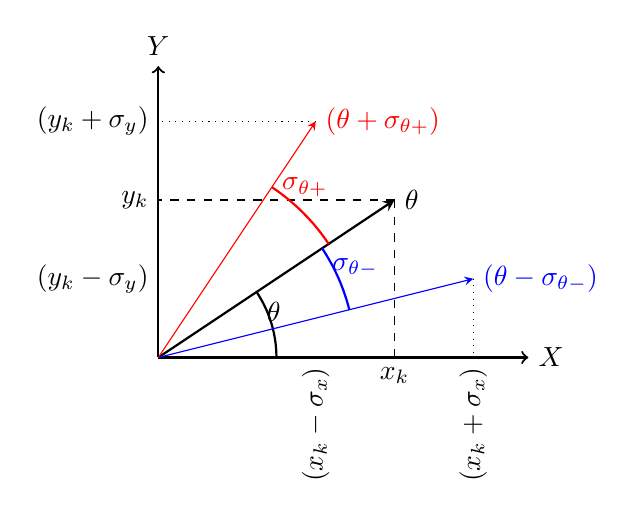
\begin{tikzpicture}
			\def \accX {3}
			\def \accY {2}
			\def \sigmaAccX {1}
			\def \sigmaAccY {1}
			\def \Xaxis {\accX+\sigmaAccX+0.7}
			\def \Yaxis {\accY+\sigmaAccY+0.7}
			%
			% Define angles
			% It is very important to get redundant parenthesis
			\pgfmathsetmacro{\bottomAngle}{atan(((\accY-\sigmaAccY)) / ((\accX+\sigmaAccX)))}
			\pgfmathsetmacro{\mediumAngle}{atan(((\accY)) / ((\accX)))}
			\pgfmathsetmacro{\upperAngle}{atan(((\accY+\sigmaAccY)) / ((\accX-\sigmaAccX)))}
			%
			% Draw coordinate system
			\draw[thick,->](0,0) -- (\Xaxis,0) node[right]{$X$};
			\draw[thick,->](0,0) -- (0,\Yaxis) node[above]{$Y$};
			%
			% Draw arrow medium position
			\draw[thick,-stealth](0,0) -- (\accX,\accY) node[right]{$\theta$};
			% Draw medium point
			\draw[dashed] (\accX,\accY) -- (\accX,0) node[below] {$x_k$};
			\draw[dashed] (\accX,\accY) -- (0,\accY) node[left] {$y_k$};
			% Draw angle
			\def \radiusMediumAngle {1.5}
			\draw[thick,black] ([shift=(0:\radiusMediumAngle)]0,0) arc (0:\mediumAngle:\radiusMediumAngle)node[below right]{$\theta$};
			\pause
			% Draw horizontal SD
			\draw[dotted] (\accX+\sigmaAccX,\accY-\sigmaAccY) -- (\accX+\sigmaAccX,0) node[rotate=90,left]{$(x_k+\sigma_x)$};
			\node[rotate=90,left] at (\accX-\sigmaAccX,0) {$(x_k-\sigma_x)$};
			\pause
			% Draw vertical SD
			\node[left] at (0,\accY-\sigmaAccY) {$(y_k-\sigma_y)$};
			\draw[dotted] (\accX-\sigmaAccX,\accY+\sigmaAccY) -- (0,\accY+\sigmaAccY) node[left]{$(y_k+\sigma_y)$};
			\pause		
			% Draw arrow bottom position
			\draw[-stealth,blue](0,0) -- (\accX+\sigmaAccX, \accY-\sigmaAccY) node[right]{$(\theta-\sigma_{\theta -})$};
			% Angle. Syntax: (startingPointX,startingPointY) arc (startAngle:stopAngle:radius)
			% ([shift=(t:r)] x, y) is the proper starting point, where (x,y) is the center and (t:r) is the polar coordinate of starting point.
			\def \radiusBottomAngle {2.5}
			\draw[thick,blue] ([shift=(\bottomAngle:\radiusBottomAngle)]0,0) arc (\bottomAngle:\mediumAngle:\radiusBottomAngle)node[below right]{$\sigma_{\theta -}$};
			\pause
			% Draw arrow upper position
			\draw[-stealth,red](0,0) -- (\accX-\sigmaAccX, \accY+\sigmaAccY) node[right]{$(\theta+\sigma_{\theta +})$};
			% Angle
			\def \radiusUpperAngle {2.6}
			\draw[thick,red] ([shift=(\mediumAngle:\radiusUpperAngle)]0,0) arc (\mediumAngle:\upperAngle:\radiusUpperAngle)node[right]{$\sigma_{\theta +}$};
			\end{tikzpicture}
		\end{figure}
		\onslide<6->{
			\begin{equation}
			(\theta_z - \sigma_{\theta -}) = \arctan \frac{y_k-\sigma_y}{x_k+\sigma_x}
			,\quad
			(\theta_z + \sigma_{\theta +}) = \arctan \frac{y_k+\sigma_y}{x_k-\sigma_x}
			\end{equation}}
		\onslide<7->{
			\begin{equation}\label{eq:sigmaPlusMinus}
			\sigma_k =(\sigma_{\theta +} + \sigma_{\theta -}) = \arctan \frac{y_k+\sigma_y}{x_k-\sigma_x} - \arctan \frac{y_k-\sigma_y}{x_k+\sigma_x}
			\end{equation}
		}
	\end{frame}
		
\end{document}